\clearpage
\section{Operational sidequest: quantum mechanics in subsystem composition}
\label{sec:f1-operational}

\textbf{7 September 2026.} We now have a concrete positive candidate for
the subsystem-first programme. Its endpoint assigns
\[
\mathcal A(S)=\mathbb C[\operatorname{Sym}(S)]
\]
to a finite set of constituents. The algebras have normalized positive
states, CP dynamics, Born probabilities and proper assembly inclusions.
One constituent has only scalar observables; three constituents have an
$M_2(\mathbb C)$ sector. Two disjoint three-constituent clusters can carry
a Bell state. The construction is a quantum family, not a proposed
single-particle wavefunction over a one-element coefficient field.

The arithmetic precursor is the positive type-A Hecke family. At finite
field cardinality $q$, it is the invariant transition algebra of complete
flags in a chosen configuration Lagrangian. Two overlapping subsystem
embeddings determine $q\geq1$ through the intrinsic Born overlap
$q/(q+1)^2$, even though their abstract algebra types are independent of $q$.
The endpoint at one is an actual specialization of algebraic presentations.

The limitation is explicit: this is a \emph{flag-context sector extracted
from polarized Weyl quantum mechanics}. It is not yet a specialization of
the entire Weyl algebra, its phase data and every change of polarization.
The research report is \path{docs/sidequests/f1-operational.md}.

\subsection{A positive arithmetic family}

\begin{definition}[Hecke systems and their reference trace]
Fix a real $q>0$. Put $H_0(q)=H_1(q)=\mathbb C$. For $n\geq2$, define
the unital complex algebra $H_n(q)$ by generators $T_1,\ldots,T_{n-1}$,
involution $T_i^*=T_i$, and relations
\[
(T_i-q)(T_i+1)=0,\qquad
T_iT_{i+1}T_i=T_{i+1}T_iT_{i+1},\qquad
T_iT_j=T_jT_i\quad(|i-j|>1).
\]
For $w\in S_n$, let $T_w$ be a reduced-word product and let $\ell(w)$
be its Coxeter length. Define the coefficient functional by
$\tau_n(T_w)=\delta_{w,1}$.
\end{definition}
\begin{scope}Basis independence, positivity and the C*-norm are proved
below. The real parameter becomes a field cardinality only at the
specified arithmetic fibres.\end{scope}
\provenance{D1101}{definitions.md}{f1\_operational\_check.py (H1,H2)}{f1-operational-adjudication.md}

\begin{theorem}[Positive Hecke quantum algebras]
{\normalfont\statusProved}\quad For every $q>0$ and $n\geq0$, the
$T_w$ form a basis of $H_n(q)$, $T_w^*=T_{w^{-1}}$, and
\[
\tau_n(T_u^*T_v)=\delta_{u,v}q^{\ell(u)}.
\]
Consequently $\tau_n$ is a faithful normalized positive trace, and left
multiplication on $L^2(H_n(q),\tau_n)$ gives a faithful finite C*-algebra
representation.
\end{theorem}
\begin{scope}This covers all positive real parameters, including one.
It does not assert positivity at arbitrary complex roots of unity.\end{scope}
\provenance{F1-HCK-POS}{f1-operational/hecke.md, section 1}{H1,H2}{f1-operational-adjudication.md}
\begin{proof}
On a basis $b_w$, the standard generator raises Coxeter length with
coefficient one, and on a descent acts by
$q b_{s_iw}+(q-1)b_w$. The two-string matrix is
$\left(\begin{smallmatrix}0&q\\1&q-1\end{smallmatrix}\right)$.
The rank-two strings verify the defining relations. Reduced words span
and are independent by their action on $b_1$. With
$\langle b_u,b_v\rangle=\delta_{u,v}q^{\ell(u)}$, every generator is
self-adjoint. This proves the Gram identity and
$\tau_n(x^*x)=\sum_w|x_w|^2q^{\ell(w)}$. The basis identity also gives
traciality. The faithful regular *-representation has closed finite-dimensional image.
\end{proof}

\begin{definition}[Finite-field flag context algebra]
Fix a named finite field $k=\mathbb F_Q$ and an $n$-dimensional $k$-space
$L$. A complete flag is $0=U_0<U_1<\cdots<U_n=L$ with
$\dim_kU_i=i$. Put
\[
\operatorname{Cxt}(L)=\operatorname{End}_{GL(L)}\ell^2(\operatorname{Fl}(L)).
\]
Let $(A_wf)(F)=\sum_{\operatorname{pos}(F,F')=w}f(F')$, labelling
relative positions by reduced gallery words in adjacency-product order.
Use the normalized operator trace
$\operatorname{tr}_{\rm Fl}(a)=|\operatorname{Fl}(L)|^{-1}\operatorname{Tr}(a)$.
If $L$ is a named configuration Lagrangian of a Weyl system, call this
its complete-flag context algebra.
\end{definition}
\begin{scope}The context register is a separate Hilbert space from the
Weyl configuration register. The Lagrangian is named data.\end{scope}
\provenance{D1104}{definitions.md}{H9}{f1-operational-adjudication.md}

\begin{theorem}[Arithmetic realization by invariant flag transitions]
{\normalfont\statusProved}\quad For every finite field $\mathbb F_Q$
and finite-dimensional $L$ of dimension $n$, the adjacency map
$T_w\mapsto A_w$ is a trace-preserving *-isomorphism
\[
H_n(Q)\simeq\operatorname{Cxt}(L).
\]
\end{theorem}
\begin{scope}The operator convention is direct; a right-convolution
convention would require the usual opposite/inversion adjustment.\end{scope}
\provenance{F1-HCK-FLAG}{f1-operational/hecke.md, section 2; Iwahori 1964}{H9, fields of orders 2 and 3}{f1-operational-adjudication.md}

This is the finite-field construction in
\href{https://repository.dl.itc.u-tokyo.ac.jp/records/39909}{Iwahori (1964)},
Lemma 3.1 and Theorems 3.2 and 4.1. Pair-orbits of flags are indexed by
$S_n$ and their kernels span the commutant. An adjacent panel contains
$Q+1$ flags, so its nonidentity adjacency has square
$Q I+(Q-1)A_{s_i}$. Transposition inverts relative position, and only
the identity kernel has nonzero diagonal. These facts fix the trace.

\begin{definition}[Ordered assembly and coarse graining]
For real $q>0$ and $m,n\geq0$, embed $S_m\times S_n$ as consecutive block permutations
in $S_{m+n}$. Define
\[
\iota_{m,n}(T_u\otimes T_v)=T_{u\times v},\qquad
E_{m,n}(T_w)=
\begin{cases}T_w,&w\in S_m\times S_n,\\0,&\text{otherwise},\end{cases}
\]
identifying the retained basis with $H_m(q)\otimes H_n(q)$.
\end{definition}
\begin{scope}These are ordered maps. No symmetric block swap is stipulated
at $q\ne1$.\end{scope}
\provenance{D1102}{definitions.md}{H3}{f1-operational-adjudication.md}

\begin{theorem}[Coherent positive assembly]
{\normalfont\statusProved}\quad For $q>0$ and $m,n\geq0$, $\iota_{m,n}$
is an injective unital trace-preserving *-homomorphism. The map $E_{m,n}$
is the unique faithful trace-preserving UCP conditional expectation onto
its image. Both families satisfy ordered three-block coherence.
\end{theorem}
\begin{scope}Complete positivity includes all matrix amplifications.
The finite checker samples this statement; the proof has no rank bound.\end{scope}
\provenance{F1-HCK-TOWER}{f1-operational/hecke.md, section 3}{H3,H13, stated finite samples}{f1-operational-adjudication.md}
\begin{proof}
The two sets of block generators commute and their basis images are
distinct. The coefficient trace restricts to the product trace.
Orthogonality of the basis makes $E$ the trace-orthogonal projection.
The trace-pairing characterization gives its bimodule property and
positivity; repeating the projection argument in every matrix amplification
gives complete positivity. The two three-block routes retain precisely
$S_l\times S_m\times S_n$. The classical source for the expectation is
\href{https://doi.org/10.2748/tmj/1178245177}{Umegaki (1954)}.
\end{proof}

\begin{definition}[Operational states and processes of a Hecke level]
Fix real $q>0$ and $n\geq0$. A state is a positive functional $\omega:H_n(q)\to\mathbb C$ with
$\omega(1)=1$, represented by $h\geq0$, $\tau_n(h)=1$, through
$\omega(a)=\tau_n(ha)$. An effect satisfies $0\leq e\leq1$ and has
probability $\tau_n(he)$. Deterministic Heisenberg channels are UCP;
outcome maps are subunital CP and an instrument has a unital sum.
The ordered product density is $\iota_{m,n}(h\otimes k)$.

A retained local Kraus list satisfies $\sum_iK_i^*K_i=1$ and gives
\[
\Phi_K(a)=\sum_iK_i^*aK_i,\qquad
\mathcal T_K(h)=\sum_iK_ihK_i^*.
\]
In a larger block, embed the operators before applying these formulas.
\end{definition}
\begin{scope}Equality of isolated CP maps is not assumed to survive
assembly. Not every CP map is asserted to have this local inner form.\end{scope}
\provenance{D1106}{definitions.md}{H3,H5,H8}{f1-operational-adjudication.md}

\begin{theorem}[Quantum operational semantics of the positive family]
{\normalfont\statusProved}\quad For $q>0$, the Hecke states have unique
positive normalized densities, effects give Born probabilities, and the
stated restriction and preparation maps are CP. Ordered product densities
are normalized and associative. Retained local Kraus processes extend
coherently through ordered block assembly.
\end{theorem}
\begin{scope}This is a finite C*-quantum sector. A tensor law on arbitrary
isolated CP shadows has not been asserted.\end{scope}
\provenance{F1-HCK-OPS}{f1-operational/hecke.md, section 4}{H3,H5,H8}{f1-operational-adjudication.md}

The density/functional identification is blockwise matrix duality for a
faithful trace. The equality
\[
\tau_{m+n}\bigl(\iota(h\otimes k)a\bigr)
=(\omega_h\otimes\omega_k)(E_{m,n}(a))
\]
identifies product preparation with precomposition by the conditional
expectation. Positivity and normalization give the Born interval $[0,1]$.

\subsection{The parameter lives in the subsystem diagram}

\begin{definition}[Unlabelled overlap and marked trace]
Let a finite C*-algebra have a unique noncommutative simple summand
$M_2(\mathbb C)$ and two specified unital subalgebras $B_1,B_2\simeq
\mathbb C^2$. When the two pairs of minimal projections compress to
rank-one projections in that block, define
\[
a(\mathcal A;B_1,B_2)=\min_{P\in B_1,\,Q\in B_2}\operatorname{Tr}_2(PQ),
\]
where the minimum runs over those compressed minimal projections and
$\operatorname{Tr}_2$ is ordinary matrix trace. Separately, in $H_2(q)$
define $e_{\rm triv}=(T_1+1)/(q+1)$ and $r_2=\tau_2(e_{\rm triv})$.
\end{definition}
\begin{scope}The first invariant does not label the projections or use a
chosen reference state. The second invariant explicitly marks the trivial
projection.\end{scope}
\provenance{D1103,D1105}{definitions.md}{H4}{f1-operational-adjudication.md}

\begin{theorem}[Arithmetic memory in overlapping subsystems]
{\normalfont\statusProved}\quad For every $q>0$,
\[
H_1(q)=\mathbb C,\quad H_2(q)\simeq\mathbb C^2,\quad
H_3(q)\simeq\mathbb C^2\oplus M_2(\mathbb C).
\]
For the left and right $H_2$ inclusions in $H_3$, the unlabelled overlap is
\[
a(q)=\frac{q}{(q+1)^2},\qquad
q=\frac{1-2a+\sqrt{1-4a}}{2a}\quad(q\geq1).
\]
It determines exactly $\{q,q^{-1}\}$, and uniquely determines $q$ on
$q\geq1$. The marked trace instead satisfies $r_2=1/(q+1)$ and determines
$q$ without that range restriction.
\end{theorem}
\begin{scope}The algebra types alone do not determine the parameter.
The two overlapping embeddings, or the separately marked trace, do.\end{scope}
\provenance{F1-HCK-LOW,F1-HCK-Q}{f1-operational/hecke.md, sections 5--6}{H4,H5}{f1-operational-adjudication.md}

In the matrix block one may calculate with
\[
P_1=\begin{pmatrix}1&0\\0&0\end{pmatrix},\qquad
P_2=\begin{pmatrix}a&\sqrt{a(1-a)}\\\sqrt{a(1-a)}&1-a\end{pmatrix}.
\]
The four unlabelled overlaps are $a,a,1-a,1-a$, and $a\leq1/4$.
This matrix calculation proves a basis-independent statement about the
abstract C*-diagram. The reciprocal *-isomorphism is
$T_i\mapsto-qS_i$ into $H_n(q^{-1})$.

\begin{figure}[htbp]
\centering
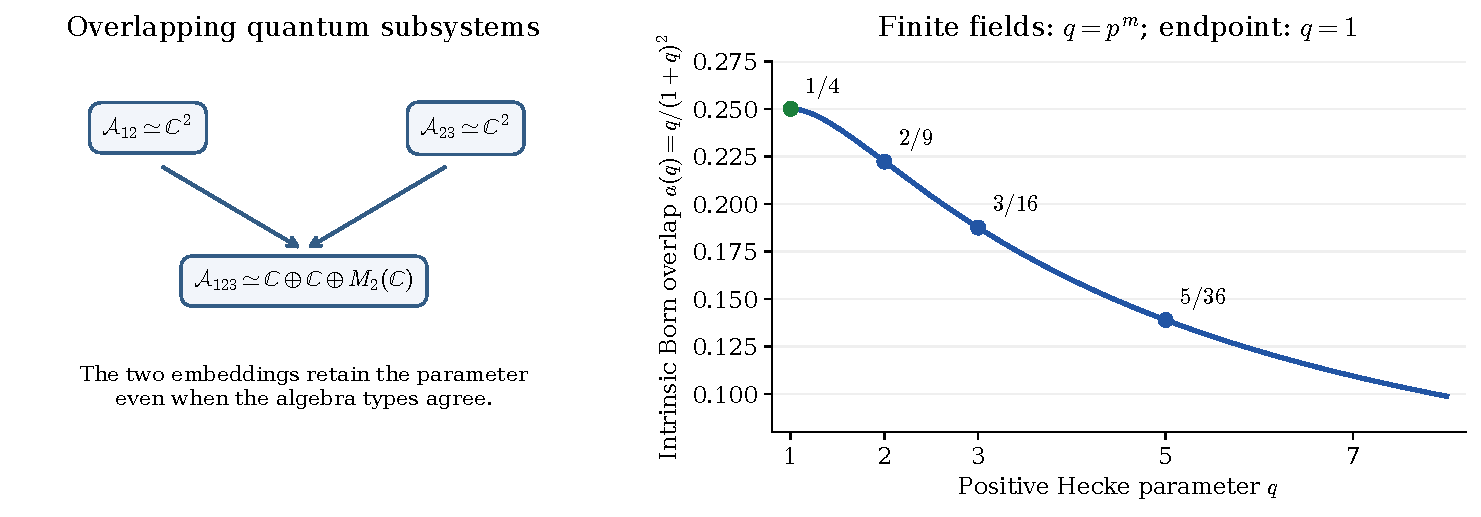
\includegraphics[width=\linewidth]{figures/f1-operational-overlap.pdf}
\caption{The abstract algebra types stay fixed, while the relative subsystem
embeddings retain the positive parameter. The markers are exact rational
probabilities; the intervening curve illustrates the proved formula.}
\label{fig:f1-operational-overlap}
\end{figure}

The coefficient trace on $H_3(q)$ is
\[
\tau_3(a_+,a_-,a_{\rm std})=
\frac{a_++q^3a_-}{(q+1)(q^2+q+1)}
+\frac{q}{q^2+q+1}\operatorname{Tr}_2(a_{\rm std}).
\]
Thus a standard-block pure state with ordinary density $P_2$ has full
density $h=P_2/\gamma$, $\gamma=q/(q^2+q+1)$. Let
$u_1=2e_1-1$, $e_1=(T_1+1)/(q+1)$. Its isolated action on the left
commutative $H_2$ is identity, but the same retained unitary in $H_3$
changes the return probability for effect $P_2$ from $1$ to
\[
(1-2a(q))^2.
\]
At one the full density is $3P_2$ and the return probability is $1/4$.
Preparing it by measuring $P_2$ in the reference state has success
probability $1/3$. This is a complete finite quantum experiment.

\subsection{A functor on normal maps over the field with one element}

\begin{definition}[The symmetric-group quantum net]
For a finite set $S$, put $G(S)=\operatorname{Sym}(S)$ and
$\mathcal A(S)=\mathbb C[G(S)]$, with
\[
\Bigl(\sum_ga_gg\Bigr)^*=\sum_g\overline{a_g}g^{-1},\qquad
\tau_S\Bigl(\sum_ga_gg\Bigr)=a_1.
\]
An injection $f:S\to T$ extends permutations by the identity off $f(S)$,
giving $i_f$. Its reverse coefficient map $E_f$ deletes terms outside
that subgroup. Disjoint union gives the block inclusion $\mu_{S,T}$.
States use $h\geq0$, $\tau_S(h)=1$, and $\omega_h(a)=\tau_S(ha)$.
Local Kraus lists satisfy $\sum_iK_i^*K_i=1$; their action in $T$ retains
the embedded list $i_f(K_i)$. Lists are identified under scalar unitary
mixing after padding by zero operators.
\end{definition}
\begin{scope}The coefficient trace is normalized. It is different from
the unnormalized categorical trace used later for a general fusion category.\end{scope}
\provenance{D1125}{definitions.md}{H5,H7,H8}{f1-operational-adjudication.md}

\begin{theorem}[A collective quantum endpoint]
{\normalfont\statusProved}\quad The symmetric-group assignment on finite
injections, with its coefficient expectations, states and retained local
Kraus processes, is a finite quantum net. It has coherent proper
disjoint assembly and CP restriction/preparation. Its three-constituent
standard sector has the full density $3P_2$ and the Born witness $1\to1/4$.
\end{theorem}
\begin{scope}The net supplies a sufficient coherent class of local
processes, not a canonical extension of every isolated CP map.\end{scope}
\provenance{F1-OP-SYM}{f1-operational/cp.md, CPOP-5}{H5,H7,H8}{f1-operational-adjudication.md}

\begin{definition}[Partial-injection realization]
A normal map of finite pointed $\mathbb F_1$ modules preserves the
basepoint and has at most one preimage of each non-basepoint. On nonzero
sets it is a partial injection $f:S\rightharpoonup T$, a bijection
$D\to E$ between subsets. Define
\[
\mathcal R(f)=i_{E\subset T}\circ\mathcal A(f:D\simeq E)\circ E_{D\subset S}.
\]
The target has finite tracial C*-algebras, unital trace-preserving CP
maps and trace adjoints as daggers. Wedge of pointed modules becomes
disjoint union of the nonzero sets.
\end{definition}
\begin{scope}This is the normal-map convention; arbitrary pointed maps
are not included.\end{scope}
\provenance{D1010,D1127}{definitions.md; Szczesny 1204.5395}{H12}{f1-operational-adjudication.md}

\begin{theorem}[Operational realization of normal F1 maps]
{\normalfont\statusProved}\quad On finite sets and partial injections
$f:D\subseteq S\to E\subseteq T$, put $\mathcal A(S)=\mathbb C[\operatorname{Sym}(S)]$
with coefficient trace, and
$\mathcal R(f)=i_E\mathcal A(f:D\simeq E)E_D$, using subgroup inclusion
and coefficient expectation. This functor is dagger and lax symmetric
monoidal, with structure maps
\[
\mu_{S,T}:\mathcal A(S)\otimes\mathcal A(T)
\hookrightarrow\mathcal A(S\sqcup T).
\]
An empty partial map has image $a\mapsto\tau_S(a)1_T$.
\end{theorem}
\begin{scope}The laxators need not be isomorphisms. The source zero map
is a reference reset, not zero CP; this is a nonadditive functor.\end{scope}
\provenance{F1-OP-PMAP}{f1-operational/contexts.md, PMAP-1}{H12}{f1-operational-adjudication.md}
\begin{proof}
A group-basis permutation survives precisely when its support is in
$D$; then it is relabelled and extended by identity. Two successive
survival conditions say that the support lies in the domain of the
composed partial map. This proves functoriality. Inclusion and coefficient
expectation are trace adjoints, proving the dagger statement. The same
support calculation proves naturality under disjoint union; associativity
and symmetry follow from the canonical set bijections.
\end{proof}

The source wedge operation is therefore collective assembly. Classical
alternatives can separately use C*-algebra direct sums, with their
central probabilities. They are not the same operation, and neither
should be silently identified with unrestricted coherent Hilbert direct sum.

\subsection{An exact process quotient and a sharp context bound}

\begin{definition}[Kraus Gram and contextual equivalence]
Fix a nonempty finite $S$, $n=|S|$, $H=\operatorname{Sym}(S)$, and
normalized local lists. Write $K_i=\sum_ha_i(h)h$ and put
\[
J_K(h,k)=\sum_i a_i(h)\overline{a_i(k)}.
\]
Two lists are contextually equivalent when their Heisenberg maps
$\Phi_{K,f}(a)=\sum_i i_f(K_i)^*a\,i_f(K_i)$ agree after every finite
injection into an ambient set. Stable scalar-unitary equivalence pads
lists by zeros and applies a unitary matrix to the Kraus index.
An admissible Gram is $J\geq0$ with
\[
\sum_hJ(hx,h)=\delta_{x,1}\qquad(x\in H).
\]
\end{definition}
\begin{scope}The Gram is process data, not just the isolated CP action.
It has trace one by the constraint at $x=1$.\end{scope}
\provenance{D1126}{definitions.md}{H8,H11}{f1-operational-adjudication.md}

\begin{theorem}[Finite contextual recovery of a quantum process]
{\normalfont\statusProved}\quad Fix a finite set $S$ of size $n\geq1$
and finite lists in $\mathbb C[\operatorname{Sym}(S)]$ normalized by
$\sum_iK_i^*K_i=1$, extended through permutation inclusions along finite
injections $S\to T$. Kraus Gram equality, stable scalar-unitary equivalence and equality of
all ambient CP actions are equivalent. One ambient set of size $2n-1$
suffices. For $n\geq2$ this universal size bound is sharp, with explicit
positive-state Born witnesses.
\end{theorem}
\begin{scope}The theorem concerns retained local Kraus processes of
the symmetric-group net. It is not a claim about every structural partial
map or every quantum channel in every fusion category.\end{scope}
\provenance{F1-OP-KCF}{f1-operational/contexts.md, KCF-1}{H11 at q=1}{f1-operational-adjudication.md}
\begin{proof}
In an ambient set of size $2n-1$, choose an involution $g$ exchanging
$n-1$ local points with the outside points and fixing the remaining one.
Then $H\cap gHg^{-1}=1$, so all words $h^{-1}gk$ are distinct. The expansion
\[
\Phi_K(g)=\sum_{h,k}J_K(k,h)h^{-1}gk
\]
recovers every Gram coefficient. Conversely equal Grams give equal
maps in all contexts. Equality of finite Grams gives exactly stable
unitary mixing by extending an isometry between coefficient-vector spans.

For sharpness let $p_+,p_-$ be the local trivial and sign central
projections and $p_0=1-p_+-p_-$. The normalized lists
$(p_++p_-,p_0)$ and $(p_+-p_-,p_0)$ differ only in cross terms between
the trivial and sign sectors. In every smaller possible ambient set,
each support intersection has at least two points. Its transposition
forces those cross terms to vanish. At size $2n-1$ they do not vanish.
For $e=(1+g)/2$, set $\Delta=\Phi_+(e)-\Phi_-(e)$.
Both images are effects and have equal trace, so $h=1+\Delta$ is a
positive normalized density, with Born difference $\tau(\Delta^2)>0$.
\end{proof}

Thus $n-1$ ancillary constituents can be necessary. At $n=2$ all inner
channels are the isolated identity on $\mathbb C^2$, while their Grams
form the disk
\[
J=\begin{pmatrix}r&ib\\-ib&1-r\end{pmatrix},\qquad b^2\leq r(1-r).
\]
A three-constituent context distinguishes them. The corresponding
positive-Hecke context-bound extension remains \statusSketch{}: its
minimal-double-coset argument is written down and exact examples at
$q=2$, $n=2,3$ pass, but only the symmetric-group theorem was admitted.
\provenance{F1-OP-KCF-Q}{f1-operational/contexts.md, separated extension}{H11 at q=2}{supporting SKETCH}

\subsection{The partial-flag category is explicitly constructible}

\begin{definition}[Partial-flag corners and their specialization]
Fix real $q>0$. A composition $\alpha=(\alpha_1,\ldots,\alpha_r)$ of $n$ has positive
parts summing to $n$; include the empty composition of zero. Let
$W_\alpha$ preserve its consecutive blocks and put
\[
P_\alpha(q)=\sum_{w\in W_\alpha}q^{\ell(w)},\qquad
e_\alpha=P_\alpha(q)^{-1}\sum_{w\in W_\alpha}T_w.
\]
Define $\Gamma_q(\alpha,\beta)=e_\beta H_n(q)e_\alpha$ for equal
totals, and zero Hom spaces for different totals. Composition is
multiplication, identity is $e_\alpha$, adjoint is $*$, and tensor
concatenates compositions through $\iota$. Let $x=(1)$. Finite formal
sums and splitting self-adjoint idempotents give the additive completion;
only its nonzero objects are used as normalized quantum systems.
The generic coefficient ring is
$\mathbb Z[t,t^{-1},\{P_\alpha(t)^{-1}\}_\alpha]$, evaluated at $t=q$.

For $L=\mathbb F_Q^n$, partial flags have successive quotient dimensions
$\alpha$. If $r_\alpha$ forgets steps, define
\[
J_\alpha e_E=P_\alpha(Q)^{-1/2}\sum_{F:r_\alpha(F)=E}e_F.
\]
The normalized corner trace is $\tau_\alpha=P_\alpha(q)\tau_n$.
A corner Kraus family $v_j\in e_\beta H_n e_\alpha$ is normalized when
$\sum_jv_j^*v_j=e_\alpha$ and acts by $a\mapsto\sum_jv_j^*av_j$.
\end{definition}
\begin{scope}The localization is explicit. There is no rigidity or
cross-degree preparation in the amplitude category itself.\end{scope}
\provenance{D1141}{definitions.md}{H9,H13}{supporting SKETCH}

\begin{proposition}[A positive monoidal category of flag contexts]
{\normalfont\statusSketch}\quad For $q>0$, $\Gamma_q$ is a graded
monoidal C*-category. At a finite field cardinality $Q$, its corner
morphisms are exactly the $GL(L)$ intertwiners between partial-flag
Hilbert spaces, through $a\mapsto J_\beta^*aJ_\alpha$.
Refinement is represented by the corresponding typed projection.
At one,
\[
\operatorname{End}_{\Gamma_1}(x^{\otimes n})=\mathbb C[S_n],
\]
the C-linear finite-bijection skeleton, with partial-flag retracts added.
\end{proposition}
\begin{scope}An operational envelope supplies normalized states and
additional preparations. The corner trace rescaling must be retained.\end{scope}
\provenance{F1-OP-FLAGCAT}{f1-operational/flag-category.md, sections 1--3}{H9,H13}{supporting SKETCH}

The calculation is elementary: $T_s\sum_{W_\alpha}T_w=q\sum_{W_\alpha}T_w$
implies $e_\alpha^2=e_\alpha=e_\alpha^*$. Block length additivity gives
$\iota(e_\alpha\otimes e_\beta)=e_{\alpha\mathbin{\|}\beta}$.
Refinement gives $e_\beta e_\alpha=e_\beta$, and
$J_\alpha J_\alpha^*=e_\alpha$. A density transported by a corner Kraus
family uses the factor $P_\alpha/P_\beta$ between the two normalized traces.

\subsection{A concrete coupling back to Weyl quantum mechanics}

\begin{definition}[Weyl constraint flags and controlled tests]
Fix $k=\mathbb F_Q$ of characteristic $p$, an $n$-dimensional named
configuration Lagrangian $L$, and nontrivial additive
$\psi:k\to U(1)$. On $\mathbb C[L]$ use
$X(u)e_y=e_{y+u}$ and $Z(\chi)e_y=\chi(y)e_y$, with additive characters
$\chi:L\to U(1)$; the $k$-linear dual is identified through $\psi$.
For a $k$-subspace $U$, let $U^{\rm ann}$ be the characters trivial on it
and define
\[
P_U^X=|U|^{-1}\sum_{u\in U}X(u),\qquad
P_U^Z=|U^{\rm ann}|^{-1}\sum_{\chi\in U^{\rm ann}}Z(\chi).
\]
On $K_{\rm ctx}(L)=\mathbb C[\operatorname{Fl}(L)]$, declare the flag
basis orthonormal and put, on its tensor with the Weyl register,
\[
C_i=\sum_F|F\rangle\langle F|\otimes P_{U_i(F)}^Z.
\]
The Levi action is $R(g)e_y=e_{gy}$, together with permutation of flags.
\end{definition}
\begin{scope}The field, Lagrangian, origin and phase datum are retained.
The context and Weyl Hilbert spaces are different registers.\end{scope}
\provenance{D1142}{definitions.md}{character identities in the proof}{supporting SKETCH}

\begin{proposition}[Flags as quantum constraint chains]
{\normalfont\statusSketch}\quad Fix a finite field $k=\mathbb F_Q$, an
$n$-dimensional configuration Lagrangian $L$ and a nontrivial additive
character $\psi:k\to U(1)$. Its complete flags inject $GL(L)$-equivariantly
into each of the two nested Weyl projector chains, with commutation
within each chain. The $C_i$ are commuting orthogonal
projections on the joint context/Weyl register, invariant under the
diagonal Levi action.
\end{proposition}
\begin{scope}This is an extraction and coupling of sectors. It is not an
equivalence with full Weyl quantum mechanics or a proof of independence
from the polarization.\end{scope}
\provenance{F1-HCK-CONTEXT,F1-OP-COUPLE}{f1-operational/flag-category.md, section 4}{explicit character derivation}{supporting SKETCH}

Character orthogonality gives $P_U^Z=\sum_{y\in U}|y\rangle\langle y|$;
$P_U^X$ averages on cosets. The two projector-chain ranks are $Q^i$ and
$Q^{n-i}$. These formulas make the coupling explicit, while the dimensions
$Q^n$ and $[n]_Q!$ prevent an unmentioned identification of the two registers.

\begin{definition}[Coordinate-apartment comparison]
For a finite field $\mathbb F_Q$, $L=\mathbb F_Q^n$ and an ordered basis of $L$, embed the coordinate
complete flags by the isometry $J_{\rm ap}:\mathbb C[S_n]\to
\mathbb C[\operatorname{Fl}(L)]$, using the gallery/regular-action convention.
Put $\Omega_Q(a)=J_{\rm ap}^*aJ_{\rm ap}$ on the context commutant.
\end{definition}
\begin{scope}This is an operational comparison at a fixed field, not
the definition of substituting one into parameter-dependent coefficients.\end{scope}
\provenance{D1144}{definitions.md}{H9 apartment probes}{supporting SKETCH}

\begin{proposition}[A direct CP map from arithmetic contexts to the endpoint]
{\normalfont\statusSketch}\quad For every prime power $Q$, apartment
compression is basis-independent after permutation labelling and gives
a trace-preserving UCP map $H_n(Q)\to\mathbb C[S_n]$, $T_w\mapsto w$.
It commutes with ordered block inclusions and coefficient expectations.
\end{proposition}
\begin{scope}For $Q>1$ it is not multiplicative and is not automatically
natural for every partial-flag corner compression.\end{scope}
\provenance{F1-OP-APART}{f1-operational/flag-category.md, section 7}{H9 at Q=2,3}{supporting SKETCH}

Each relative position has one neighbour within the coordinate apartment.
Changing its basis conjugates by $GL(L)$, which fixes the commutant.
These facts prove the range and independence; isometric compression proves
complete positivity. The limits are visible in
$\Omega_Q(T_s^2)=(Q-1)s+Q1\ne1=\Omega_Q(T_s)^2$.
A coarse flag compression gives scalar $Q$ before the apartment map
but scalar one after it. Compatible refinement-process comparison is
therefore a concrete remaining problem.

\subsection{The broader categorical operational framework}

\begin{definition}[Nonzero categorical subsystem data]
Let $\mathcal C$ be a unitary fusion category with its positive spherical
trace and a tensor-closed replete family of nonzero objects containing
the unit. Define
\[
A_X=\operatorname{End}_{\mathcal C}(X),\quad
d_X=\operatorname{Tr}_X(1_X)>0,\quad
\tau_X=\operatorname{Tr}_X/d_X,
\]
and $j_{X,Y}(a\otimes b)=a\otimes b\in A_{X\otimes Y}$.
Retain associators and the trace-preserving assembly expectations,
including their iterated comparison maps. A state has density
$\rho\geq0$, $\operatorname{Tr}_X(\rho)=1$, representing
$\omega(a)=\operatorname{Tr}_X(\rho a)$; effects lie between zero and one.
Assembly restriction is the expectation and product-subalgebra
preparation embeds its density by $j$.
\end{definition}
\begin{scope}Zero objects are excluded from normalized state systems.
This definition uses unnormalized categorical trace, unlike the coefficient
trace convention of the group net.\end{scope}
\provenance{D1121,D1122}{definitions.md}{finite expectation examples H3}{f1-operational-adjudication.md}

\begin{theorem}[Positive assembly without a strong Hilbert fibre]
{\normalfont\statusProved}\quad Let $\mathcal C$ be a unitary fusion category
with its positive spherical trace and a tensor-closed replete family of
nonzero objects containing the unit. Then $A_X=\operatorname{End}_{\mathcal C}(X)$
are finite C*-algebras with faithful
positive traces. Assembly is injective and trace-multiplicative and has
a unique UCP trace-preserving expectation. States, restriction,
preparation and Born probabilities are well defined and coherent under
nested assembly.
\end{theorem}
\begin{scope}No strong monoidal Hilbert-space fibre functor is required.
The inclusion may be proper.\end{scope}
\provenance{F1-OP-ALG}{f1-operational/cp.md, CPOP-1--2}{H3, examples only}{f1-operational-adjudication.md}

In simple-sector coordinates,
$A_X=\bigoplus_aM_{m_a}(\mathbb C)$ and
$\operatorname{Tr}_X=\sum_a d_a\operatorname{Tr}_{m_a}$, with $d_a>0$.
This proves faithfulness and identifies the quantum-trace weights.
The expectation is orthogonal projection for the trace inner product;
matrix amplification proves its complete positivity. The relevant
internal operator-algebra analogue is developed by
\href{https://arxiv.org/abs/1611.04620}{Jones--Penneys}; their internal
algebra objects are not being identified with this net without a comparison.

\begin{definition}[Retained categorical Kraus and dilation processes]
Let $\mathcal C$ be a unitary fusion category with positive spherical trace,
and fix a tensor-closed replete family of nonzero objects containing the unit.
For family objects $X,Y$, a Kraus process is a finite list
$K_i:X\to Y$ with $\sum_iK_i^*K_i=1_X$, modulo stable scalar-unitary
mixing. It acts by $\Phi_K(a)=\sum_iK_i^*aK_i$ and
$\mathcal T_K(\rho)=\sum_iK_i\rho K_i^*$; its retained right-context
operators are $K_i\otimes1_Z$. Composition uses $L_jK_i$, and tensor
uses $K_i\otimes L_j$, with the category associators.

A charge-carrying dilation is a named nonzero environment $E$ and
isometry $v:X\to Y\otimes E$, with
$\Phi_v(a)=v^*(a\otimes1_E)v$. Sequential composition retains its
ordered environment. Parallel composition requires named unitary
interchange, supplied for example by a unitary braiding or a specified
environment half-braiding.
\end{definition}
\begin{scope}Not every isolated CP map is asserted to be represented
by these local lists, and arbitrary environments are not silently
interchangeable in a merely monoidal category.\end{scope}
\provenance{D1123,D1124}{definitions.md}{H8; finite examples}{f1-operational-adjudication.md}

\begin{theorem}[Coherent quantum processes from retained operators]
{\normalfont\statusProved}\quad In a unitary fusion category with positive
spherical trace, fix a tensor-closed replete family of nonzero objects
containing the unit. On that family,
normalized Kraus lists compose and tensor modulo stable scalar-unitary
mixing. Their shadows are UCP and their density maps preserve categorical
trace in every retained context. The stated dilations compose sequentially
and in parallel when the named interchange data are provided.
\end{theorem}
\begin{scope}This does not quotient by equality of isolated shadows.
That coarser identification fails in the examples above.\end{scope}
\provenance{F1-OP-PROC}{f1-operational/cp.md, CPOP-3}{H8}{f1-operational-adjudication.md}

The essential identity is
$\sum_{i,j}K_i^*L_j^*L_jK_i=1_X$; cyclicity gives trace preservation.
Scalar unitary mixing cancels the Kraus indices in every context. These
are the data that an isolated CP map can fail to retain.

For comparison, use the standard unitary Fibonacci data
\[
\varphi=\frac{1+\sqrt5}{2},\qquad
F=\begin{pmatrix}\varphi^{-1}&\varphi^{-1/2}\\
\varphi^{-1/2}&-\varphi^{-1}\end{pmatrix},\qquad
R=\operatorname{diag}(e^{-4\pi i/5},e^{3\pi i/5}).
\]
On the two-anyon algebra $\mathbb C^2$, $\operatorname{Ad}_R$ is identity.
In the charge-$\tau$ matrix block of three anyons it is nontrivial:
the $|+\rangle$ return probability becomes $(5-\sqrt5)/8$.
The braid $FRF$ has $|0\rangle$ return probability $(3-\sqrt5)/2$.
These sourced comparisons remain \statusSketch{} and do not identify
Fibonacci with the arithmetic endpoint.
\provenance{F1-OP-FIB}{f1-operational/cp.md, CPOP-4; Ahmadi--Kissinger 2211.03855}{independent exact critic recomputation}{supporting SKETCH}

\subsection{Entanglement and alternative branches}

\begin{definition}[A Bell density on two collective sectors]
In $\mathbb C[S_3]$, let $s=(12)$, $t=(23)$,
$z=(2-(123)-(132))/3$, and put
$Z_*=zs$, $X_{\rm num}=z(s+2t)$, $Y_{\rm anti}=z(st-ts)$.
For the block inclusion into $\mathbb C[S_6]$, define
\[
P_{\rm Bell}=\frac14\mu\left(
z\otimes z+Z_*\otimes Z_*+
\frac{X_{\rm num}\otimes X_{\rm num}+Y_{\rm anti}\otimes Y_{\rm anti}}3
\right),\qquad h_{\rm Bell}=9P_{\rm Bell}.
\]
On the standard sector the normalized observables are $Z_*$ and
$X_*=X_{\rm num}/\sqrt3$.
\end{definition}
\begin{scope}The coefficient trace on the full six-constituent algebra
fixes the density factor nine.\end{scope}
\provenance{D1143}{definitions.md}{H14}{supporting SKETCH}

\begin{proposition}[A Bell state of two disjoint collective qubits]
{\normalfont\statusSketch}\quad The stated $P_{\rm Bell}$ is a positive
projection, $\tau_6(h_{\rm Bell})=1$, and both subgroup marginals are
$(3/2)z$, the maximally mixed standard-sector qubit states. Its $XX$ and
$ZZ$ correlations are one and its crossed correlations zero, giving the
ordinary CHSH value $2\sqrt2$ with the corresponding qubit measurements.
\end{proposition}
\begin{scope}This uses two disjoint size-three regions and their local
matrix blocks; it does not assert that all composite observables factor locally.\end{scope}
\provenance{F1-OP-BELL}{f1-operational/flag-category.md, section 6}{H14}{supporting SKETCH}

In the standard block $X_{\rm num}=\sqrt3X$ and
$Y_{\rm anti}=i\sqrt3Y$, so the formula is the usual Bell projector.
Each standard block contributes trace weight $1/3$; their product gives
$1/9$. The conditional expectation extends the Bell functional to the
full composite while preserving these local correlations.

The type-C flag route remains distinct: at one its signed permutation
groups have a rank-two $D_8$ qubit sector, but
$B_m\times B_n$ is not parabolic in $B_{m+n}$. A separate assembly theorem
is needed. The rank-two Temperley--Lieb route also needs extra input:
its coefficient is $\delta^{-2}=q/(q+1)^2$, with
$\delta=\sqrt q+1/\sqrt q$. At one it gives the $SU(2)$ spin tensor-power
centralizer tower after the quotient and a Jones/Markov trace. The
faithful flag trace cannot descend through the nonzero quotient: at level
two the flag weights are $(1/2,1/2)$, whereas spin singlet/triplet weights
are $(1/4,3/4)$. Full rigidity additionally requires duality conventions.
The Fibonacci quotient is a different root-of-unity construction with
its corresponding positive star/trace structure.

The substantive outcome is a quantum subsystem family with intrinsic
arithmetic memory, an explicit positive endpoint and a sharp description
of its process data. The remaining central task is comparison with the
full Weyl system and all its refinement/polarization processes. Those
missing comparisons are stated as such; they are not hidden inside the
word ``canonical.''
